\documentclass[border=10pt]{standalone}
\usepackage{tikz}
\usepackage[margin=1in]{geometry}
\usepackage{amsmath}
\usetikzlibrary{positioning, arrows.meta, decorations.pathmorphing, patterns, calc, shadows.blur}

\begin{document}

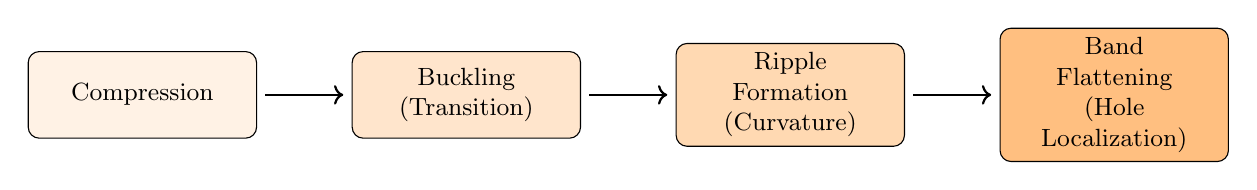
\begin{tikzpicture}[
node distance=1.3cm and 1.2cm,
every node/.style={
draw,
rectangle,
rounded corners,
minimum height=1.1cm,
minimum width=2.9cm,
align=center,
font=\small,
text=black
},
shorten >=3pt, shorten <=3pt
]
\node[fill=orange!10!white] (comp) {Compression};
\node[fill=orange!20!white, right=of comp] (buck) {Buckling\\(Transition)};
\node[fill=orange!30!white, right=of buck] (ripple) {Ripple\\Formation\\(Curvature)};
\node[fill=orange!50!white, right=of ripple] (flat) {Band\\Flattening\\(Hole\\Localization)};
\foreach \i/\j in {comp/buck, buck/ripple, ripple/flat}
\draw[->, thick] (\i) -- (\j);
\end{tikzpicture}


\end{document}
